\section{Билет 21. Теорема Лиувилля для гармонических функций (случай $\R^3$)}
% Затехал: Дмитрий Федоряка

\subsection{Формулировка теоремы} 

\begin{theorem}

{\bf (Теорема Лиувилля)} Функция $u(x)$, гармоническая в $\R^3$ ($\Delta u = 0$)  и имеющая на бесконечности рост не выше степенного (т.е. $|u(x)| \le C (1+|x|)^{\mu}$), является многочленом от $x_1,x_2,x_3$ степени не выше $\mu$.

\end{theorem}

\subsection{Доказательство при $\mu \ge 0$}

Общая идея - доказать, что все производные степени выше $\mu$ равны нулю.


\begin{enumerate}



\item{

Выберем $x \in \R^3, R>0$ так, чтобы $R > 2|x|$:
\begin{center}
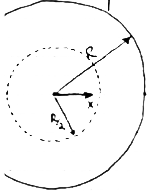
\includegraphics{21_1_new}
\end{center}
В области $|x|<R$ $u(x)$ - гармоническая, а $\left. u(x) \right|_{\partial \Omega} \in C(\partial \Omega)$.

Тогда применима формула Пуассона для шара:

$$u(x) = \frac{1}{4 \pi R} \oint_{|y|=R}{\frac{R^2-|x|^2}{|y-x|^3} u(y) dS_y }
$$

В силу выбора $R$ имеем $|y-x| \ge |y|- |x| \ge \frac{R}{2} >0$.

Можем записать:

$$\mathcal{D}_{x}^{\alpha} u(x) = \frac{1}{4 \pi R} 
\oint_{|y|=R}{\mathcal{D}_{x}^{\alpha}\roundBr{\frac{R^2-|x|^2}{|y-x|^3}}u(y) dS_y}$$

}





\item{

Докажем по индукции, что
 
$$\forall \alpha = (\alpha_1,\alpha_2,\alpha_3)~~~ \mathcal{D}_{x}^{\alpha}\squareBr{\frac{R^2-|x|^2}{|x-y|^3}} = \frac{P_{\alpha}(R,x,y)}{|x-y|^{3+2|\alpha|}},$$

где $P_\alpha$ - однородный многочлен степени $|a|+2$ от $R, x_1,x_2,x_3,y_1,y_2,y_3$.


\begin{itemize}
	\item {База:}
	
	$$\mathcal{D}_{x}^{(0,0,0)}\squareBr{\frac{R^2-|x|^2}{|x-y|^3}} = \frac{R^2-x_1^2-x_2^2-x_3^2}{|x-y|^3}$$
	
	\item {Переход. 
Пусть требуемое верно $\forall \alpha: |a|\le k$. Возьмём $\hat{\alpha}=(\alpha_1+1, \alpha_2, \alpha_3)$:}

$$
\mathcal{D}_{x}^{\hat{\alpha}}\squareBr{\frac{R^2-|x|^2}{|x-y|^3}} = \frac{\partial}{\partial x_1}
\squareBr{\frac{P_{\alpha}(R,x,y)}{|x-y|^{3+2|\alpha|}}}
=
\frac{
\frac{\partial P_{\alpha}}{\partial x_1} \cdot |x-y|^2 - (3+2|\alpha|)\cdot P_\alpha \cdot (x_1-y_1)
}
{|x-y|^{3+2(|\alpha|+1)}}
=
\frac{P_{\hat{\alpha}}(R,x,y)}{|x-y|^{3+2|\hat{\alpha}|}}
$$ 
	
\end{itemize}
}



\item{
Покажем теперь, что $\forall |x| \le \frac{R}{2}, \Forall |y|=R, \Forall \alpha =(\alpha_1,\alpha_2,\alpha_3)$ справедлива оценка:

$$\left| \mathcal{D}_{x}^{\alpha}\roundBr{\frac{R^2-|x|^2}{|x-y|^3}} \right| \le \frac{C_\alpha}{R^{1+|\alpha|}}.
$$

Действительно, $|P_\alpha| \le \tilde{C}_\alpha R^{|a|+2}$, а $|x-y|^{3+2|\alpha|} \ge \roundBr{\frac{R}{2}}^{3+2|\alpha|} = \hat{C_\alpha}R^{3+2|\alpha|}$. Отсюда следует требуемая оценка.
}

\item{

Теперь докажем, что $\mathcal{D}_x^\alpha u(x) = 0 \Forall \alpha\colon |\alpha|>\mu$.

$$
\left| \mathcal{D}_x^{\alpha} u(x) \right| = \frac{1}{4 \pi R} 
\left|
\oint_{|y|=R}{\mathcal{D}_x^{\alpha}\roundBr{\frac{R^2-|x|^2}{|y-x|^3}}u(y)dS_y}
\right|
\le
\frac{1}{4 \pi R} \cdot C \cdot (1+ |x|)^\mu \cdot 
\frac{C_\alpha}{R^{1+|a|}} \cdot 4 \pi R^2 
\le$$ 
$$
\le
\frac{C \cdot C_\alpha \cdot (1+R)^\mu}{R^{|\alpha|}} 
\underset{R \to \infty}{\longrightarrow}
0 ~~
\text{Значит,}~~ \mathcal{D}_x^{\alpha} u(x)=0 \Forall x \in \R^3, |\alpha|>\mu .$$

} 


\item{

Для гармонической в $\R^3$ функции $u(x)$ справедливо представление:

$$
u(x) = u(0) + \sum_{k=1}^{m} \sum_{|\alpha|=k} \frac{1}
{\alpha_1! \alpha_2! \alpha_3!} \mathcal{D}_x^{\alpha} u(0) 
x_1^{\alpha_1}x_2^{\alpha_2}x_3^{\alpha_3}
+
\sum_{k=m+1}^{\infty} \sum_{|\alpha|=k} \frac{1}
{\alpha_1! \alpha_2! \alpha_3!} \underset{=0}{\mathcal{D}_x^{\alpha} u(0)}
x_1^{\alpha_1}x_2^{\alpha_2}x_3^{\alpha_3}
=
$$

$$
=
u(0) + \sum_{k=1}^{m} \sum_{|\alpha|=k} \frac{1}
{\alpha !} \mathcal{D}_x^{\alpha} u(0) 
x^{\alpha},
$$

где $m = [\mu], \alpha ! \triangleq \alpha_1!\alpha_2!\alpha_3!, x^\alpha \triangleq x_1^{\alpha_1}x_2^{\alpha_2}x_3^{\alpha_3}$.



}

\end{enumerate}






\subsection{Доказательство при $\mu < 0$}

Пусть $\mu<0$. Тогда т.к. $|u(x)|\le C(1+|x|)^\mu, \mu<0$, то
$|u(x)| \le C (1+|x|)^0 \equiv C_1$. 

По предыдущему пункту, $u(x)$ - полином степени 0, т.е. константа.

Но $|u(x)| \le \frac{C}{(1+|x|)^{|\mu|}} \Rightarrow u(x) 
\underset{|x| \to \infty}{\longrightarrow}
0   \Rightarrow u(x) \equiv 0$.
 
